\begin{landscape}
\subsection{Experiment Components}
\subsubsection{Electrical Components}

Table \ref{tab:electrical-components} shows all required electrical components with mass and price.

%


\begin{longtable}{|m{0.03\textwidth}|m{0.3\textwidth}|m{0.25\textwidth}|m{0.05\textwidth}|m{0.1\textwidth}|m{0.3\textwidth}|m{0.15\textwidth}|m{0.08\textwidth}|}
    
\hline
\textbf{ID} & \textbf{Components} & \textbf{Specs (size,weight)} & \textbf{No.} & \textbf{Cost} & \textbf{Note} & \textbf{Availability} & \textbf{Status} \\ 
\hline
1 & Arduino Due & 101.52 mm x 53.3 mm, 36 g & 1 & 35 Euro & Fast and has many analog, and digital pins & Easily ordered online & Ordered \\ \hline
2 & W5500 Ethernet Shield  & 36 g & 1 & 28 Euro & Easily, connected on top of the board & Easily ordered online & Ordered \\ \hline
3 & KNF 850.1.2. KNDC B Miniature Diaphragm Pump & 30 x 54.3 x 77.5 mm, 430g  & 1 & 350 Euro & Low power, small size & Ordered online & Ordered \\ \hline
4 & Barometric Pressure Sensor MS5607-02BA03 & 5.0 x 3.0 x 1.0 mm, 1g  & 3 &  11 Euro & High resolution, large measuring range & Easily ordered online & To be ordered online \\ \hline
5 & Electromagnetically controlled valve & 1-1/2", 2640 g & 12 & 1756 Euro & Cascaded/series of valves & Easily ordered online & One ordered for testing \\ \hline
6 & Airflow sensor AWM40000 Series & 14 g & 1 & 106 Euro & good temperature range, high accuracy & Easily ordered online & To be ordered online \\ \hline
7 & Polyimide Thermofoil Heaters HK5161R78.4L12 & 12.7 x 101.6 mm, 6.84g & 1 & 40 Euro & Easy to mount, compact size & Easily ordered online & To be ordered online \\ \hline
8 & Polyimide Thermofoil Heaters HK5160R157L12 & 12.7 x 50.8 mm, 6.84g & 1 & 40 Euro & Easy to mount, compact size & Easily ordered online & To be ordered online \\ \hline
9 & Temperature sensor VSSOP-8, LM75A, Texas Instruments & 5.3 x 3.4 x 1.4 mm & 12 & 4 Euro & I2C digital output interface, temperature range down to - 55 ℃ & Easily ordered online & To be ordered online \\ \hline
10 & DC-DC Converter TEN 5 Series, 6 W, 12 V & 20.3 x 31.8 mm, 33.8 g & 3 & 50 Euro & Provides required output voltage and power & Easily ordered online & To be ordered online \\ \hline
11 & HDC2010 Low Power Humidity Digital Sensors & 1.5 x 1.5 x 0.675 mm, 15g & 1 & 3 Euro & I2C interface, good temperature range, high accuracy & Easily ordered online & To be ordered online \\ \hline
12 & Industrial temperature microSD XCUHS-I 8GB & 15 x 11 x 1 mm, 0.5 g & 1 & 20 Euro & Small, good temperature range, sufficient storage & Easily ordered online & Ordered  \\ \hline
13 & Logic CAT5E Network (2m) & 2 m, 90g & 1 & 7 Euro & Will be used for testing & Easily ordered in the nearest store & To be bought \\ \hline
14 & Electrical wires & 30g &  30 & 15 Eur & For use in testing and the final PCB board and circuitry & Easily ordered online & To be ordered \\ \hline
15 & Heat sinks & 25g &  5 &  5 Eur & For dissipating heat generated from components & Easily ordered online & To be ordered \\ \hline
16 & Resistors & 15g & 3 & 1.5 Eur & For use in valve switching circuit & Easily ordered online & To be ordered \\ \hline
17 & Transistors & 18g & 18 & 9 Eur &  For use in valve switching circuit & Easily ordered online & To be ordered \\ \hline 


    \caption{Table showing all required electrical components}
    \label{tab:electrical-components}
\end{longtable}
\raggedbottom

\begin{table}[H]
    \begin{align*}
        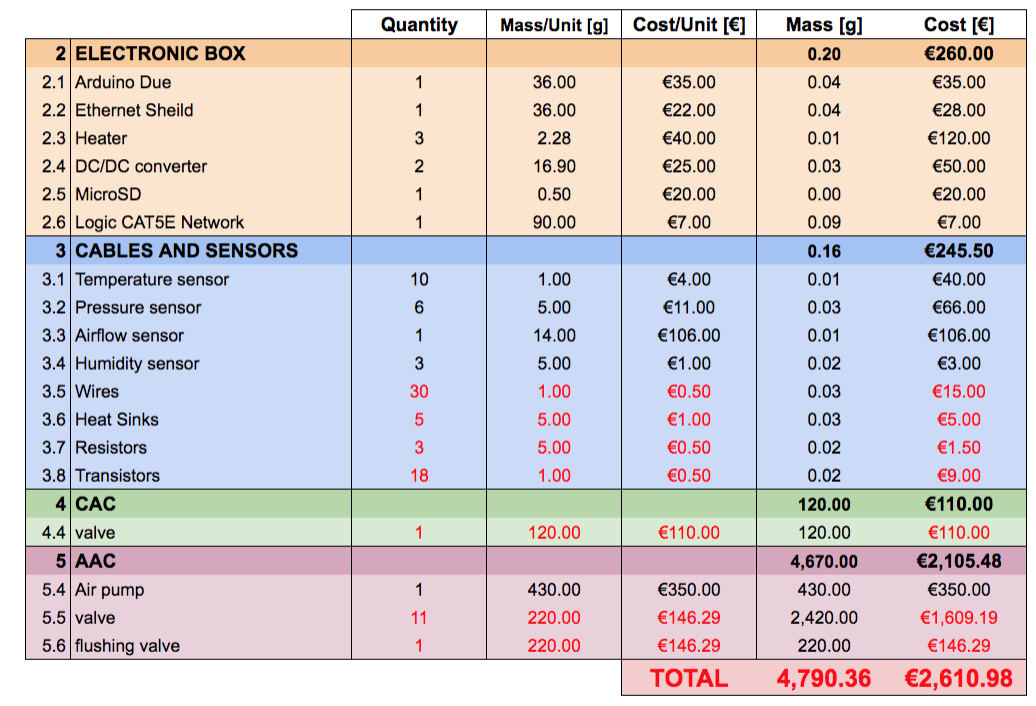
\includegraphics[height=10cm]{4-experiment-design/img/electrical-components-table.png}
    \end{align*}
    \caption{Table showing all required electrical components.}\label{tab:electrical-components}
\end{table}

\end{landscape}

\begin{landscape}

\subsubsection{Mechanical Components}

Table \ref{tab:mechanical-components} shows all required mechanical components with mass and price. Table cells highlighted in yellow denote values that have yet to be determined.

%\begin{longtable}{|m{0.03\textwidth}|m{0.2\textwidth}|m{0.25\textwidth}|m{0.05\textwidth}|m{0.1\textwidth}|m{0.28\textwidth}|m{0.15\textwidth}|m{0.15\textwidth}|}
     
   
\hline
\textbf{ID} & \textbf{Components} & \textbf{Specs (size,weight)} & \textbf{No.} & \textbf{Cost} & \textbf{Note} & \textbf{Availability} & \textbf{Status} \\ \hline
1 & Aluminum Bar & 45cm & 16 & TBD\footnote{Request for quotes have been sent to identified vendors and responses are still pending. \label{fn:mechcomp1}} & Railed geometry, Structural element & Online & To be ordered \\ \hline
2 & Aluminum Bar & 40cm & 4 & TBD\textsuperscript{\ref{fn:mechcomp1}} & Railed geometry, Structural element & Online & To be ordered \\ \hline
3 & Aluminum Bar & 25cm & 4 & TBD\textsuperscript{\ref{fn:mechcomp1}} & Railed geometry, Structural element & Online & To be ordered \\ \hline
4 & Aluminum Plate & 50 x 40 x 0.2 cm & 4 & TBD\footnote{The other elements still need to be found either in the store or online. \label{fn:mechcomp2}} & Wall, Protective element & Store & To be ordered \\ \hline
5 & Aluminum Plate & 50 x 25 x 0.2 cm & 4 & TBD\textsuperscript{\ref{fn:mechcomp2}} & Wall, Protective element & Store & To be ordered \\ \hline
6 & Aluminum Plate & 50 x 50 x 0.2 cm & 2 & TBD\textsuperscript{\ref{fn:mechcomp2}} & Wall, Protective element & Store & To be ordered \\ \hline
7 & Styrofoam & 2 $m^2$, 2.5cm thick & 1 & TBD\textsuperscript{\ref{fn:mechcomp2}} & Wall, Protective element & Store & To be ordered \\ \hline
8 & Bag Valves & \textit{Swagelok} & 16 & TBD\textsuperscript{\ref{fn:mechcomp1}} & Interface bags with tubes & Online & To be ordered \\ \hline
9 & 90-degree angle & 0.25 x 0.25 cm & 52 & TBD\textsuperscript{\ref{fn:mechcomp2}} & Join structure bars & Online & To be ordered \\ \hline
10 & Coated box & 10 x 10 x 3 cm & 1 & TBD\textsuperscript{\ref{fn:mechcomp2}} & Valve center for AAC & Store & To be built \\ \hline
11 & Plastic Tube & 5 m & 1 & TBD\textsuperscript{\ref{fn:mechcomp2}} & Valves to bags & Store & To be ordered \\ \hline
12 & Air Filter & TBD\textsuperscript{\ref{fn:mechcomp2}} & 1 & TBD\textsuperscript{\ref{fn:mechcomp2}} & Main pipe protection & Store & To be built \\ \hline
13 & Flange & Small & 50 & TBD\textsuperscript{\ref{fn:mechcomp2}} & Join tubes with valves & Store & To be ordered \\ \hline
14 & Hinges & 5 x 5 x 0.1 cm & 2 & TBD\textsuperscript{\ref{fn:mechcomp2}} & Allow opening mechanism & Store & To be ordered \\ \hline
15 & Bar & 52.4 x 0.8 cm & 4 & TBD\textsuperscript{\ref{fn:mechcomp2}} & Anchor point fro bags & Store & To be ordered \\ \hline
16 & Handle & TBD\textsuperscript{\ref{fn:mechcomp2}} & 4 & TBD\textsuperscript{\ref{fn:mechcomp2}} & Experiment box manipulation & Store & To be ordered \\ \hline

    \caption{Table showing all required mechanical components}
    \label{tab:mechanical-components}
\end{longtable}
\raggedbottom

\begin{table}[H]
    \begin{align*}
        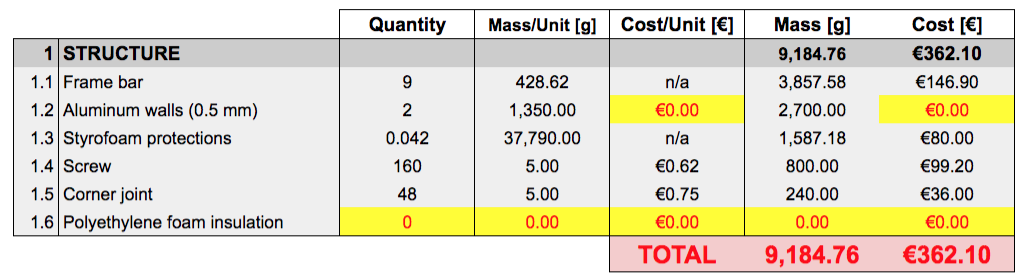
\includegraphics{4-experiment-design/img/mechanical-components-table.png}
    \end{align*}
    \caption{Table showing all required mechanical components.}\label{tab:mechanical-components}
\end{table}

\subsubsection{Other Components}

Other components are included in the full budget previously presented in Table \ref{tab:budget-table}.

\end{landscape}

\raggedbottom